% F1 -- architecture of sremu (DESIGN 13.4; WP12). Drawn at \columnwidth (252 pt).
% Every element names a committed module (checked against sremu commit 2a016a6):
%   apps / controllers: sremu.api.device (Device.inproc, Device.connect), sremu.compat,
%     sremu.transport.client, sremu.control.remote (run_remote), sremu.control.builtin
%   data plane: sremu.transport.zmq_native (TX ingress PULL, RX egress PUSH; framing.py
%     header), sremu.transport.rawreqrep (raw REQ/REP peers, lockstep only)
%   control: sremu.transport.control_server (ROUTER requests, DEALER barriers, PUB telemetry;
%     stream.open is a control request)
%   engine: sremu.engine.{emulator,scheduler,commands,barriers,pacer,streams}
%   physics: sremu.physics.propagation (snapshot, combine), channel.render_{numpy,numba}
%   recorder: sremu.record.{manifest,eventlog,sigmf,replay,report}
\documentclass[10pt,tikz,border=0pt]{standalone}
% sremu-figstyle.tex -- shared style of the TikZ diagrams F1 and F2 (WP12; DESIGN 13.4).
% Fonts: Times (newtx), as in the IEEEtran body text; every label is at least 8 pt at print
% size because the diagrams are drawn at their printed width (F1: \columnwidth = 252 pt;
% F2: \textwidth = 516 pt) and included without scaling.
% Colours: Okabe-Ito (colour-blind safe). Every colour coding is doubled by a line style
% (data plane solid, control plane dashed, recording dotted), so the diagrams also read in
% grey scale.
\usepackage[T1]{fontenc}
\usepackage{newtxtext,newtxmath}
\usepackage{tikz}
\usetikzlibrary{arrows.meta,positioning,calc,fit,backgrounds,patterns,decorations.pathreplacing}

\definecolor{okBlack}{HTML}{000000}
\definecolor{okOrange}{HTML}{E69F00}
\definecolor{okSky}{HTML}{56B4E9}
\definecolor{okGreen}{HTML}{009E73}
\definecolor{okYellow}{HTML}{F0E442}
\definecolor{okBlue}{HTML}{0072B2}
\definecolor{okVermillion}{HTML}{D55E00}
\definecolor{okPurple}{HTML}{CC79A7}

\newcommand{\figfont}{\fontsize{8}{9.4}\selectfont\hyphenpenalty=10000\exhyphenpenalty=10000}
\newcommand{\figtitle}{\fontsize{8}{9.4}\selectfont\bfseries}

\tikzset{
  every picture/.style={font=\figfont, line width=0.6pt,
    >={Stealth[length=4.5pt,width=3.6pt,line width=0pt]}},
  box/.style={draw=okBlack, rounded corners=1.5pt, align=center, inner sep=2.5pt,
    fill=white},
  app/.style={box, fill=okSky!18},
  eng/.style={box, fill=okOrange!14},
  rec/.style={box, fill=okGreen!14},
  step/.style={box, fill=okOrange!10, text width=#1},
  step/.default={5.1cm},
  ask/.style={box, fill=okSky!14, rounded corners=5pt, text width=#1},
  ask/.default={3.0cm},
  side/.style={box, fill=white, dashed, text width=#1},
  side/.default={1.9cm},
  data/.style={draw=okBlue, line width=1.0pt, ->},
  data2/.style={draw=okBlue, line width=1.0pt, <->},
  ctrl/.style={draw=okVermillion, line width=1.0pt, dash pattern=on 3pt off 1.8pt, ->},
  ctrl2/.style={draw=okVermillion, line width=1.0pt, dash pattern=on 3pt off 1.8pt, <->},
  recd/.style={draw=okGreen, line width=1.3pt, dash pattern=on 0.8pt off 1.6pt, ->},
  flow/.style={draw=okBlack, ->},
  lane/.style={draw=okBlack!55, line width=0.5pt},
  note/.style={align=left, inner sep=1pt},
}

\begin{document}
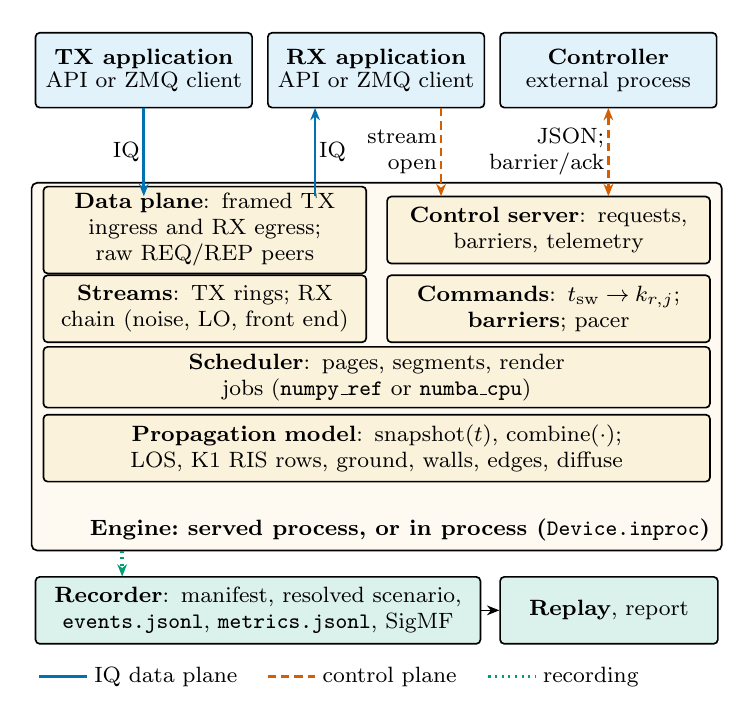
\begin{tikzpicture}[x=1cm, y=1cm]
  % fixed width: exactly \columnwidth of the IEEEtran journal class (21 pc = 252 pt)
  \useasboundingbox (0,0.02) rectangle (252pt,-8.42);

  % ---------------------------------------------------------------- external processes
  \node[app, minimum width=2.75cm, minimum height=0.95cm] (tx) at (1.475,-0.52)
    {\figtitle TX application\\[-1pt] API or ZMQ client};
  \node[app, minimum width=2.75cm, minimum height=0.95cm] (rx) at (4.425,-0.52)
    {\figtitle RX application\\[-1pt] API or ZMQ client};
  \node[app, minimum width=2.75cm, minimum height=0.95cm] (ct) at (7.375,-0.52)
    {\figtitle Controller\\[-1pt] external process};

  % ---------------------------------------------------------------- engine
  \draw[draw=okBlack, rounded corners=2pt, fill=okOrange!5] (0.05,-1.95) rectangle (8.815,-6.62);
  \node[eng, minimum width=4.1cm, text width=3.9cm, minimum height=0.85cm] (tp) at (2.25,-2.55)
    {\textbf{Data plane}: framed TX ingress and RX egress; raw REQ/REP peers};
  \node[eng, minimum width=4.1cm, text width=3.9cm, minimum height=0.85cm] (cs) at (6.615,-2.55)
    {\textbf{Control server}: requests, barriers, telemetry};
  \node[eng, minimum width=4.1cm, text width=3.9cm, minimum height=0.85cm] (st) at (2.25,-3.55)
    {\textbf{Streams}: TX rings; RX chain (noise, LO, front end)};
  \node[eng, minimum width=4.1cm, text width=3.9cm, minimum height=0.85cm] (cm) at (6.615,-3.55)
    {\textbf{Commands}: $t_{\mathrm{sw}}\!\to\!k_{r,j}$;\\ \textbf{barriers}; pacer};
  \node[eng, minimum width=8.465cm, text width=8.2cm, minimum height=0.55cm] (sc) at (4.4325,-4.42)
    {\textbf{Scheduler}: pages, segments, render jobs (\texttt{numpy\_ref} or \texttt{numba\_cpu})};
  \node[eng, minimum width=8.465cm, text width=8.2cm, minimum height=0.85cm] (pm) at (4.4325,-5.32)
    {\textbf{Propagation model}: $\mathrm{snapshot}(t)$, $\mathrm{combine}(\cdot)$;
     LOS, K1 RIS rows, ground, walls, edges, diffuse};
  \node[anchor=south east, inner sep=2pt, align=right] at (8.75,-6.58)
    {\figtitle Engine:\ served process, or in process (\texttt{Device.inproc})};

  % ---------------------------------------------------------------- recorder
  \node[rec, minimum width=5.65cm, text width=5.4cm, minimum height=0.85cm] (rc) at (2.925,-7.38)
    {\textbf{Recorder}: manifest, resolved scenario, \texttt{events.jsonl},
     \texttt{metrics.jsonl}, SigMF};
  \node[rec, minimum width=2.765cm, text width=2.5cm, minimum height=0.85cm] (rp) at (7.3825,-7.38)
    {\textbf{Replay}, report};

  % ---------------------------------------------------------------- flows
  \draw[data] (1.475,-1.0) -- node[left, note, pos=0.5] {IQ} (1.475,-2.12);
  \draw[data] (3.65,-2.12) -- node[right, note, pos=0.5] {IQ} (3.65,-1.0);
  \draw[ctrl] (5.25,-1.0) -- node[left, note, pos=0.5, align=right] {stream\\ open} (5.25,-2.12);
  \draw[ctrl2] (7.375,-1.0) -- node[left, note, pos=0.5, align=right]
    {JSON;\\ barrier/ack} (7.375,-2.12);
  \draw[recd] (1.20,-6.62) -- (1.20,-6.95);
  \draw[flow] (rc.east) -- (rp.west);

  % ---------------------------------------------------------------- legend
  \draw[data, -] (0.15,-8.22) -- (0.75,-8.22);
  \node[note, anchor=west] at (0.80,-8.22) {IQ data plane};
  \draw[ctrl, -] (3.05,-8.22) -- (3.65,-8.22);
  \node[note, anchor=west] at (3.70,-8.22) {control plane};
  \draw[recd, -] (5.85,-8.22) -- (6.45,-8.22);
  \node[note, anchor=west] at (6.50,-8.22) {recording};
\end{tikzpicture}
\end{document}
